\documentclass[xcolor=x11names,compress]{beamer}

\usepackage{graphicx}

%% Beamer Layout %%%%%%%%%%%%%%%%%%%%%%%%%%%%%%%%%%
\useoutertheme[subsection=false,shadow]{miniframes}
\useinnertheme{default}
\usefonttheme{serif}
\usepackage{palatino}

\setbeamerfont{title like}{shape=\scshape}
\setbeamerfont{frametitle}{shape=\scshape}

\setbeamercolor*{lower separation line head}{bg=DeepSkyBlue4} 
\setbeamercolor*{normal text}{fg=black,bg=white} 
\setbeamercolor*{alerted text}{fg=red} 
\setbeamercolor*{example text}{fg=black} 
\setbeamercolor*{structure}{fg=black} 
 
\setbeamercolor*{palette tertiary}{fg=black,bg=black!10} 
\setbeamercolor*{palette quaternary}{fg=black,bg=black!10} 

\renewcommand{\(}{\begin{columns}}
\renewcommand{\)}{\end{columns}}
\newcommand{\<}[1]{\begin{column}{#1}}
\renewcommand{\>}{\end{column}}
%%%%%%%%%%%%%%%%%%%%%%%%%%%%%%%%%%%%%%%%%%%%%%%%%%
\usepackage{tikz}
\usetikzlibrary{arrows}
\usetikzlibrary{decorations.pathmorphing} % wiggly line
\usetikzlibrary{positioning} % relative positioning
\usetikzlibrary{fit} % box fitting

\usepackage{adjustbox}
\usepackage{amsmath}
\usepackage{stmaryrd}
\usepackage{wasysym}
\usepackage{etoolbox}
\usepackage{separationlogic}

\begin{document}
\begin{frame}
\end{frame}

\begin{frame}[fragile]{Membrane}
\begin{columns}[c]
\column{.4\textwidth}
\begin{adjustbox}{width=\textwidth,keepaspectratio}
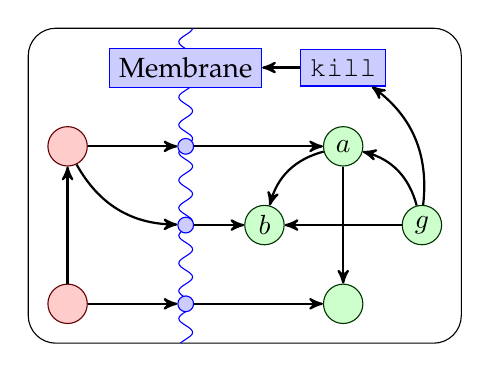
\begin{tikzpicture}[
    object/.style={circle, minimum size=5mm, inner sep=0},
    trusted/.style={object, draw=green!20!black, fill=green!20!white},
    untrusted/.style={object, draw=red!40!black, fill=red!20},
    membranec/.style={draw=blue, fill=blue!20},
    membrane/.style={object, membranec, minimum size=2mm},
    arrow/.style={thick, >=stealth'},
    pre/.style={arrow, <-},
    post/.style={arrow, ->}
  ]
  \draw[clip,rounded corners=10, use as bounding box] (0,0.5) rectangle (5.5,4.5);
  \node[trusted] (global) at (4,3) {$a$};
  \node[trusted] (a) at (3,2) {$b$}
    edge [pre,bend left] (global);
  \node[trusted] (b) at (5,2) {$g$}
    edge [post,bend right] (global)
    edge [post] (a);
  \node[trusted] (c) at (4,1) {}
    edge [pre] (global);

  \draw[membrane,decorate,decoration=snake,fill=none] (2,0) -- (2,10);
  \node[membranec,rectangle] (membrane) at (2,4) {Membrane};
  \node[membranec,rectangle] (kill) at (4,4) {\texttt{kill}}
    edge [post] (membrane)
    edge[pre,bend left] (b);
  \node[membrane] (ma) at (2,3) {}
    edge [post] (global);
  \node[membrane] (mb) at (2,2) {}
    edge[post] (a);

  \node[untrusted] (ua) at (0.5,3) {}
    edge [post] (ma)
    edge [post,bend right] (mb);
  \node[untrusted] (ub) at (0.5,1) {}
    edge [post] (ua);

  \node[membrane] (mc) at (2,1) {}
    edge [post] (c)
    edge [pre] (ub);
\end{tikzpicture}
\end{adjustbox}
\column{.6\textwidth}
{\scriptsize
\begin{verbatim}
var Membrane = function(ref) {
  var MembraneRef = function(ref) {
    var access = function(field) {
      if(!killed) {
        return MembraneRef(ref[field]);
      }
    }
    if(primitive(ref)) { return ref; }
    else { return access; }
  }

  var access = MembraneRef(ref);

  var killed = false;
  var kill = function(){ killed = true; }

  return {access: access, kill: kill};
}
\end{verbatim}
}
\end{columns}
\end{frame}

\begin{frame}
\[
\begin{array}{l}
  \{\js{y}\pointsto\_ \sep \js{x} \pointsto a \land a \bp \{\js{x}\} \}\\
  \text{[Consequence]}\\
  \{(\js{y}\pointsto\_ \sep \js{x} \pointsto a \land a \bp \{\js{x}\}) \sep (a \bp \{\js{x}\} \land \emp) \}\\
  \text{[Frame off]}\\
  \{\js{y}\pointsto\_ \sep \js{x} \pointsto a \land a \bp \{\js{x}\} \}\\
  \text{[Consequence]}\\
  \{\js{y}\pointsto\_ \sep \js{x} \pointsto a \land a \bp \{\js{x},\js{y}\} \}\\
  \js{y = x;}\\
  \{\js{y}\pointsto a \sep \js{x} \pointsto a \land a \bp \{\js{x},\js{y}\} \}\\
  \text{[Frame on]}\\
  \{(\js{y}\pointsto a \sep \js{x} \pointsto a \land a \bp \{\js{x},\js{y}\}) \sep (a \bp \{\js{x}\} \land \emp) \}\\
  \text{[Consequence]}\\
  \{\js{y}\pointsto a \sep \js{x} \pointsto a \land a \bp \{\js{x}\} \}\\
\end{array}
\]
\end{frame}
\end{document}

